\documentclass[]{memoir}

\usepackage{system/oslw-documentation}
\usepackage[hyphenate]{system/ocmc-liturgical-text} 

\def\iocDocName{AGES Liturgical Workbench (ALWB) }%

\def\iocDoc{ioc-liturgical apps }%

\def\appimages{system/images/screenshots}%

\title{User Guide\\\bigskip

\iocDocName\   (\iocDoc) \\\bigskip
}
\author{Michael Colburn\\Orthodox Christian Mission Center (OCMC)}
\date{\today}

\begin{document}

\maketitle
\tableofcontents

\vfill

\pagebreak

\chapter{Purpose of this Guide}

The purpose of this Guide is to provide information for people who use AGES Liturgical Workbench (ALWB) to create Resource Files, Template Files, and to generate services and books.

\chapter{Conventions Used in this Guide}

For this point on, the pronoun \emph{you} means the person who is the user of ALWB.

This guide will give you, the user, information you need to use ALWB.

When you see a box like the one below, it will contain an example of a tag used in an ALWB template file:

\begin{atem}
\aTag{Set}{Date} 
\aTag{month} 2
\aTag{day} 5
\aTag{year} 2017
\aTag{End}{Date}
\end{atem}

\begin{boxed}
When you see a box like this, with a blue key \color{blue}\faKey{}\color{black}, it indicates a key point.  That is, important information that will help you better understand what to do.
\end{boxed}
\begin{warning}
When you see a box like this, with a red exclamation mark in a triangle, it indicates a warning.  That is, important information that will help you avoid making a mistake.
\end{warning}

\chapter{Introduction}

AGES Initiatives, Inc. created AGES Liturgical Workbench, in partnership with the Orthodox Christian Mission Center (OCMC).  This open source software was created on behalf of the international Orthodox Christian community.  

\chapter{Creating a New Eclipse Project for ALWB}

ALWB Eclipse projects are backed up and shared usng Git and GitHub.  This chapter explains the steps to create the Git and Github repositories and create an Eclipse project in the local Git repository.

The tool used to create the repositories is GitKraken.

\begin{boxed}
GitKraken is available for Linux, Mac, and Windows.  It can be obtained at \url{https://www.gitkraken.com}.  Help on how to use GitKraken can be found at 
\url{https://support.gitkraken.com}.
\end{boxed}

The basic steps are to use GitKraken to create a Github repository and clone it to a local Git repository, then to create the project in Eclipse.  The most tricky part of the process is how to set up the directory names.

\section{Create the GitHub Repo and Local Repo}

Open GitKraken on your local machine.  Then do the following:

\begin{enumerate}
    \item Click on the white folder icon on the upper left part of the screen.
    \item Click on \emph{Init}.
    \item Click on \emph{GitHub.com}.
    \item Select the account to use, e.g. AGES-Initiatives.
    \item In the name field, enter the name of the repository, e.g. \emph{ages-alwb-library-en-us-barrett}
    \item Enter a short description, e.g. \emph{Translations by Richard Barrett.}
    \item Set the access, which normally is \emph{Public}.
    \item Assuming, for example, that \emph{c:\textbackslash git} is where you keep local git repositories, browse to that folder and select it.  Then enter the name of the repository, using the same name as entered above, e.g. \emph{ages-alwb-library-en-us-barrett}.  
    \item Set the license to Creative Commons.  
    \item Click on \emph{Create Repository and Clone}.
\end{enumerate}

\begin{warning}
The repository for an ALWB library should always start with \emph{ages-alwb-library} followed by the language code, country code, and realm, e.g. \emph{-en-us-barrett}.
\end{warning}

\section{Create the Eclipse Project}

\begin{enumerate}
    \item Open Eclipse.
    \item Click on \emph{File > New > Project > General > Project}.
    \item Click on \emph{Next}.
    \item Enter the project name, which is similar to the repository name, but not quite, e.g.: \emph{ages.alwb.library\textunderscore en\textunderscore US\textunderscore barrett}.  Note the use of dots and underscores and that the country code is in uppercase.
    \item Deselect \emph{Use default location}.
    \item Browse to the location of the repository you created using GitKraken.
    \item From there, while in the browse window, create a project directory using the same name, e.g. \emph{ages.alwb.library\textunderscore en\textunderscore US\textunderscore barrett}.
    \item Click on \emph{Open}.
    \item Click on \emph{Finish}.
    \item Right-click the new Eclipse Project, and click on \emph{Team > Disconnect}.
    \item Right-click the new Eclipse Project, and click on \emph{New > File}.  The name of the new file is \emph{.gitignore}.  
    \item Enter \emph{/.project}
    \item Save the file.
    \item Right-click the new Eclipse Project, and click on \emph{New > File}.  The name of the new file is \emph{domain.json}.  
    \item Double-click the filename to open it.  Enter \emph{\{
  "language": "en"
  , "country" : "US"
  , "realm" : "barrett"
  , "description" : "English, USA, Richard Barrett translations"
\}} using whatever the correct language, country, and realm names are, and the correct person and description.
    \item Save the file.
\end{enumerate}

\section{Adding Changes to the Repositories}

Open \emph{GitKraken}.

\begin{enumerate}
    \item In the middle pane, click on the line at the top that is a dotted circle and says \emph{WIP}, which means \emph{Work in Progress}.
    \item On the right pane, click \emph{Stage all changes}.
    \item In the bottom of the right pane, enter a short summary for the commit message.  Optionally you can enter a description.
    \item Click on \emph{Commit changes...}.
    \item On the toolbar at the top of GitKraken, click on the \emph{Push} icon.
\end{enumerate}

\chapter{Eclipse Preferences}
\section{How To Prevent Eclipse from Connecting to Git When a Project is Opened}

If you want to use Git separately from Eclipse, you will also want to prevent Eclipse from automatically connecting your project to Git when you open the project.

To do this, select:

\begin{verbatim}
    Preferences > Team > Git > Projects
\end{verbatim}

Then uncheck the box that says:

\begin{verbatim}
Automatically share projects located in a Git repository.    
\end{verbatim}
\chapter{Tags}

\section{Set\textunderscore Date End\textunderscore Date}

Purpose: gives you a way to set the date for a date-sensitive service.

Parameters:

\begin{tabular}{c|c|c}
    month & mandatory & integer 1-12\\
    day & mandatory & integer 1-31 \\
    year & optional & integer (4 numbers) 
\end{tabular}

Example: 

\begin{atem}
\aTag{Set}{Date} 
\aTag{month} 2
\aTag{day} 5
\aTag{year} 2017
\aTag{End}{Date}
\end{atem}

Description: 

A template can be used to generate a date specific service.  A template can include other templates or specified sections from other templates.  The date set for the top most template is the master date for the generation of that service.  Although included templates can temporarily change the date for rubrical purposes, when the date is reset to zero, it goes back to the master date.  That is, it resets back to the date set in the topmost template.

\begin{boxed}
The tag \aTag{Set}{Date} can be used with a Header or on a line of its own anywhere in the main body of a template. Each time it occurs, it changes the date to the one indicated.
\end{boxed}

\begin{boxed}
If you set the month and day to zero, the date will revert back to the first \aTag{Set}{Date} that the generator encountered. You do this as follows: 
\aTag{Set}{Date} 
\aTag{month} 0
\aTag{day} 0
\aTag{End}{Date}

\end{boxed}

\begin{boxed}
If in the header of a topmost template you set the month and day to zero, the date will set to today's date.  This means that if you subsequently do a reset by using \aTag{Set}{Date} 
\aTag{month} 0
\aTag{day} 0
\aTag{End}{Date}
\end{boxed}
 again, it will revert back to today's date.

\begin{warning}
Before the generator processes the lines of a template, it scans the template to find the first occurrence of a \aTag{Set}{Date}.  It will use that to set the date.  If you put a date sensitive tag before a \aTag{Set}{Date}, the generator will set the date first, then process each line of the template, including the date sensitive tag that occurred before the \aTag{Set}{Date}.
\end{warning}

\chapter{Transformer Utilities}

This chapter provides information about various utilities that can be run to transform information in one file into another file.  For example, there is a utility to transform FO files into PDF files, and HTML files in ePub files.  Each type of utility is described below in its own section.

\section{GitHub Utilities}

There are three Java files you can use to keep local repositories and Github up-to-date:

\begin{enumerate}
    \item RunToPullAllRepositories
    \item RunToResetAllRepositories
    \item RunToPushAllRepositories
\end{enumerate}

They are found in the folder \textit{net.ages.liturgical.workbench.transformer.git}.

Please read through this entire section before running them.

\subsection{Setup Common to All Three Java Files}

For each of these three classes, it is necessary that you have all your git repositories under a single parent folder. 

In each class, there in the main method, there is a variable \textit{alwbPath}.  You need to set its value to the path to the parent folder that contains allow the child repository folder.

\begin{figure}[h!]

  \begin{center}
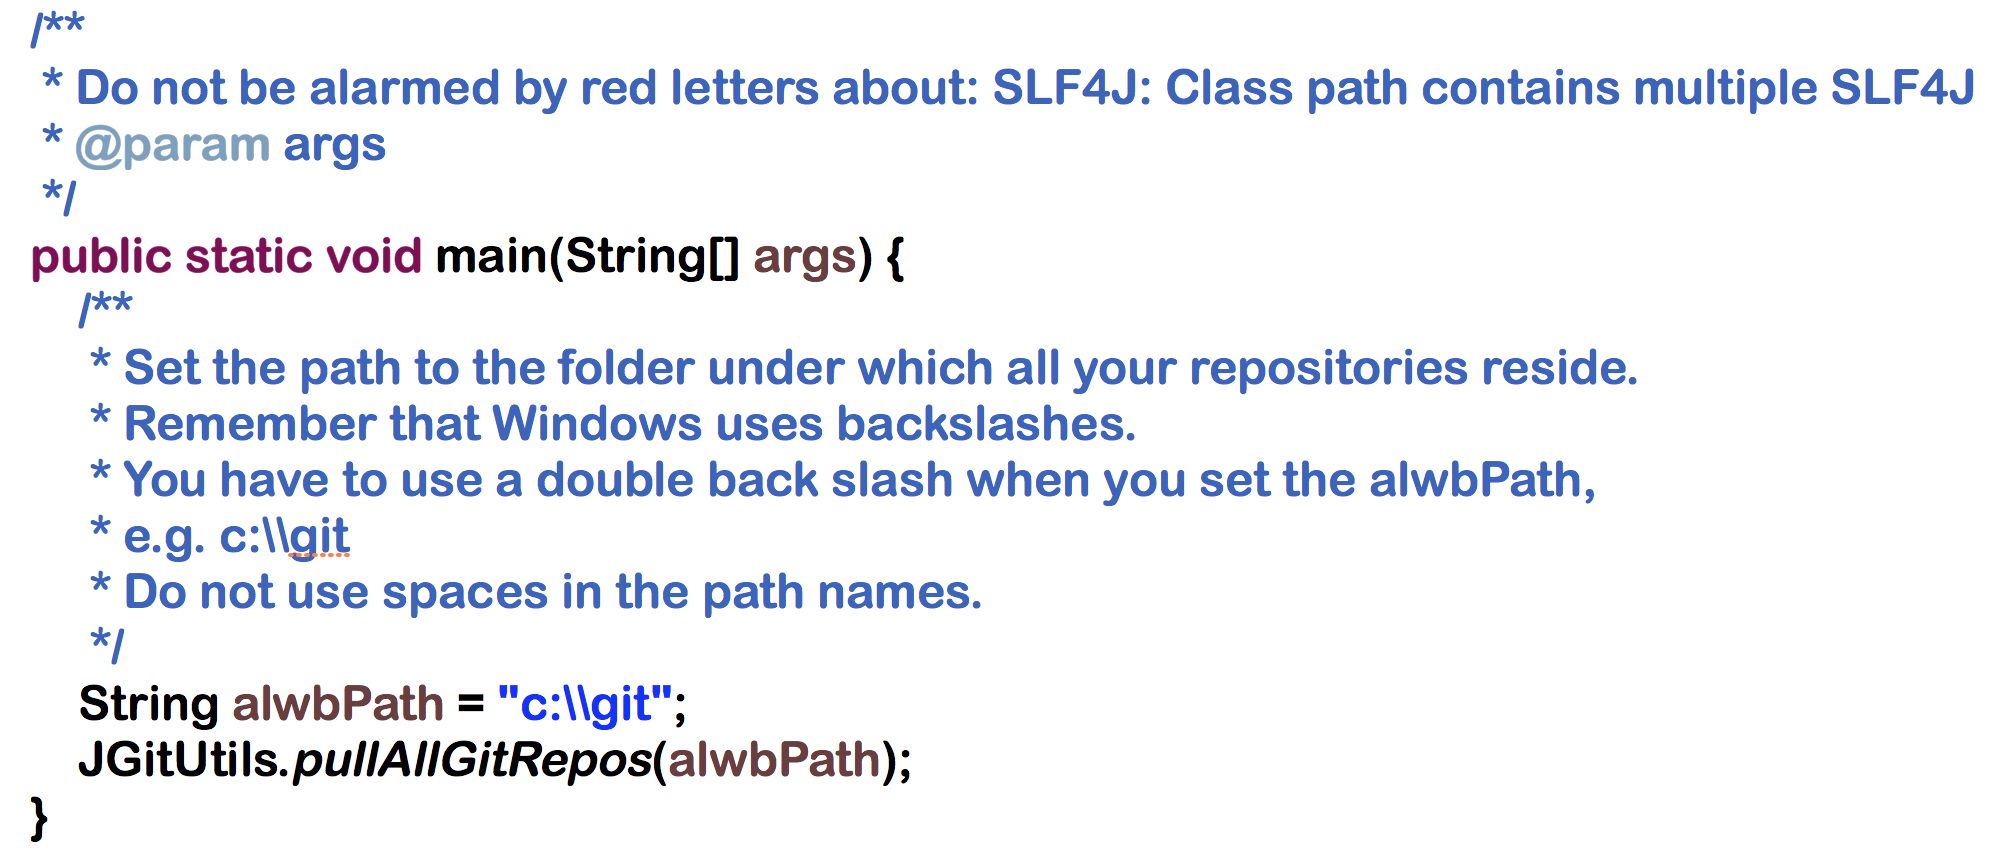
\includegraphics[scale=0.25]{alwb-user-guide/system/images/ioc-liturgical-db-public-app/alwbPath.png}
\end{center}
  \caption{The main method and the variable alwbPath}
\end{figure}

\subsection{How to Run any of the Three Java files}

For each class, you can right-click the filename and select \textit{Run as > Java Application}.

\subsection{RunToPullAllRepositories}

If you run this Java class, it will do a git pull from Github for all the repositories it finds in your parent folder.

\subsection{RunToResetAllRepositories}

If you run this Java class it will reset each repository so that it exactly matches what is currently in Github.  If you have made any changes, they will be lost.  If you have added any files that have not been committed and pushed, they will be lost.  This can, however, be very useful so that you know your repositories are identical to the ones in Github.

\subsection{RunToPushAllRepositories}

If you run this Java class, it will do the following:

\begin{enumerate}
    \item Add all files to the git index (except those excluded by the .gitignore file.
    \item Commit the files
    \item Do a pull.  This ensures that any files you have that you did not changed are up-to-date with Github.  This is important because sometimes a change occurs in Github since the last time you pulled.
    \item Push the changes to Github.
\end{enumerate}

\begin{warning}
There is extra configuration to do before you run this Java class.  See below.
\end{warning}

Before you run this Java class, you must add your Github username and password to the environmental variables.  Here is how to do this:

\begin{enumerate}
    \item Right-click the \textit{RunToPushAllRepositories.java} file and click on \textit{Properties}. 
    \item In the left pane, select \textit{Run/Debug Settings}.
    In the right pane, click the \textit{New} button.
    \item Select \textit{Java Application} and click on the \textit{OK} button.
    \item Click on the \textit{Environment} tab.  Refer to the next Figure for a screenshot.
    \item Click on the \textit{New} button.
    \item In the \textit{Name} field enter \textit{username}.  Spell it exactly like that, and all in lower case.
    \item In the value field enter your Github username.
    \item Click on \textit{OK}.
        \item Click on the \textit{New} button.
    \item In the \textit{Name} field enter \textit{pwd}.  Spell it exactly like that, and all in lower case.
    \item In the value field enter your Github password.
    \item Click on \textit{OK}.
    \item Click on \textit{OK}.
    \item Click on \textit{Apply and Close}.
\end{enumerate}

Now you can run the \textit{RunToPushAllRepositories} Java class.

\begin{figure}[h!]

  \begin{center}
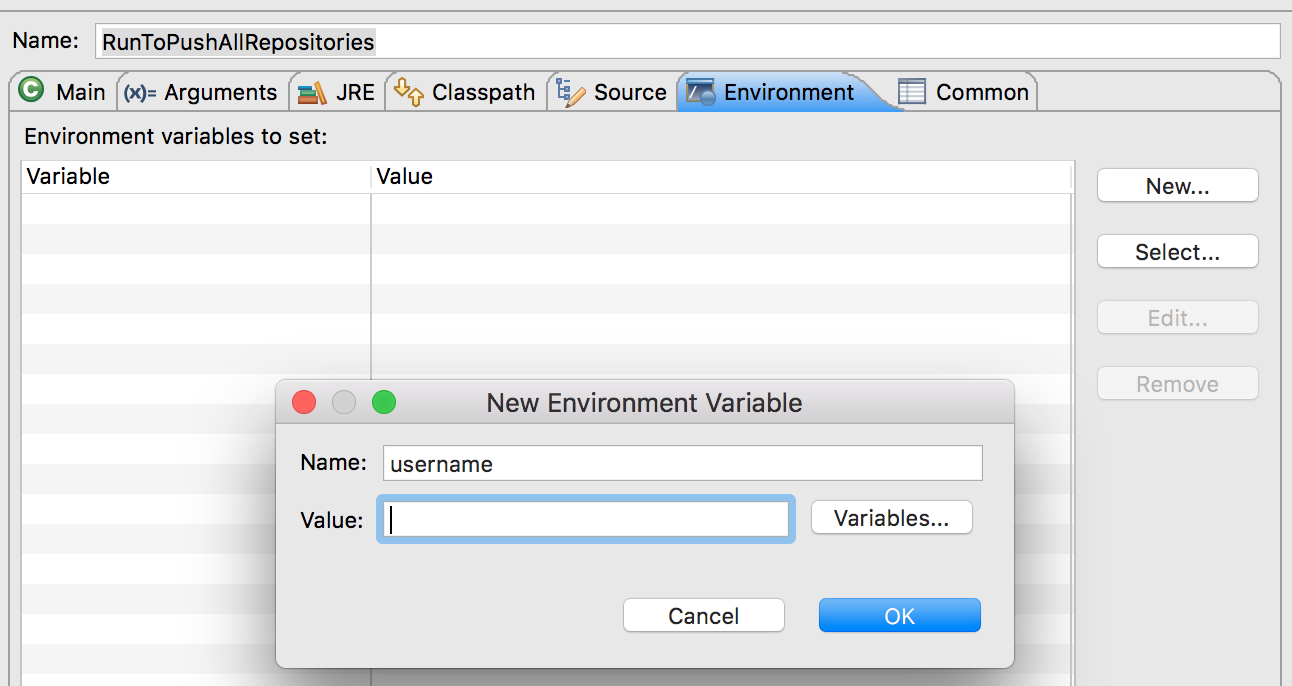
\includegraphics[scale=0.50]{alwb-user-guide/system/images/ioc-liturgical-db-public-app/envPropUsername.png}
\end{center}
  \caption{Setting environmental properties}
\end{figure}

\section{Database Synch Utility}

The \emph{Database Synch} utility is used to keep local \emph{ares} files and the \emph{IOC Liturgical Database} synchronized.  In order for synchronization to work properly, there are some steps the ALWB user must take.

\subsection{Renaming a File}
In order to update the database, it is important to preserve the information about the old filename. In order for Git to preserve this information you must do the following:

\begin{enumerate}
    \item rename the file using your usual means.  Do NOT make any other changes to the file (i.e. adding, deleting, changing, renaming key-value pairs).
    \item In your Git client (e.g. GitKraken), make sure it sees it as a file rename. 
    \item Commit the change
    \item Push the change to Github
\end{enumerate}

\begin{warning}
If you also plan to change key-values in the file, make those changes first and commit and push them to Github, before you rename the file. If you rename a file and change its contents as a single commit, Git will not keep track of what the file was previously named.  
\end{warning}

\subsubsection{Renaming a Key}

Fortunately, the Synch utility is able to detect all changes you make to ares files by reading the Git repository.  However, there is one type of change that the utility cannot reliably detect unless you help it.  

The problem is that Git will treat the rename of a key as two events: the deletion of the line that had the original key, and the insertion of a new line with the new key.  Using only information from Git, there is no reliable method for the \emph{Synch} utility to know that the deletion and insertion are in fact the renaming of a key.  For Git, this is not a problem.  But for the database, we don't want to delete the record for this key-value and add a new one.  Instead, we want to rename the key and thereby preserve other information in the database that relies on the ID of the record.

Because of this problem, if you rename an ares key, the Synch utility needs your help to know about it.

For example, lets say you have the following:

\begin{verbatim}
euCON.Key1000.title = "THE PREPARATION OF THE HOLY RELICS"    
\end{verbatim}

And, you want to rename the key \emph{euCON.Key1000.title} to \emph{euCON.Key0000.title}.

The steps you take are first, copy the current key and add it as a comment, but wrap it with the tilde character.  Second, rename the key, and save the ares file.  The end result will look like this:

\begin{verbatim}
euCON.Key0000.title = "THE PREPARATION OF THE HOLY RELICS" // ~euCON.Key1000.title~    
\end{verbatim}

That way, when the \emph{Synch} utility processes the change, it can check the comment and see if there is a key there that is wrapped in tildes.  If so, it knows that the key (on the left) is a rename from the key in the comment.  

\vfill

%==========================================
% GLOSSARY
%===========================================

\newgeometry{
top=3.5cm,
bottom=3.5cm,
left=3.7cm,
right=4.7cm,
columnsep=30pt
}

\fancyhead[L]{\textsf{\rightmark}} % Top left header
\fancyhead[R]{\textsf{\leftmark}} % Top right header
\renewcommand{\headrulewidth}{1.4pt} % Rule under the header
\fancyfoot[C]{\textbf{\textsf{\thepage}}} % Bottom center footer
\renewcommand{\footrulewidth}{1.4pt} % Rule under the footer
\pagestyle{fancy} % Use the custom headers and footers throughout the document

\newcommand{\entry}[4]{\markboth{#1}{#1}\textbf{#1}\ {(#2)}\ \textit{#3}\ $\bullet$\ {#4}}  % Defines the command to print each word on the page, \markboth{}{} prints the first word on the page in the top left header and the last word in the top right

\setlength{\parskip}{5pt}\chapter{Glossary}
%----------------------------------------------------------------------------------------

%----------------------------------------------------------------------------------------
%	SECTION A
%----------------------------------------------------------------------------------------
\begin{multicols}{2}

\section*{A}

\entry{AGES Initiatives, Inc.}{noun phrase}{}{A not-for-profit organization in the USA, founded by Fr. Seraphim Dedes. See \url{http://www.agesinitiatives.org}.}

%----------------------------------------------------------------------------------------
%	SECTION B
%----------------------------------------------------------------------------------------

\section*{B}

%----------------------------------------------------------------------------------------
%	SECTION C
%----------------------------------------------------------------------------------------

\section*{C}

\entry{country code}{noun phrase}{}{A two or three character code that identifies a specific country.  The \ltOcmcSystemAcronymn uses codes from the ISO 639-2 Code Table, that can be found at \url{https://en.wikipedia.org/wiki/ISO\textunderscore 3166-1\textunderscore alpha-3}.}

%----------------------------------------------------------------------------------------
%	SECTION D
%----------------------------------------------------------------------------------------

\section*{D}

\entry{database}{noun}{OALD}{an organized set of data that is stored in a computer and can be looked at and used in various ways. The phrase 'the database' specifically means the \iocDoc.}

\entry{domain}{noun}{}{The unique identifier of a specific version of text.  A domain has three parts: a language code, a country code, and a realm.  For example, en\textunderscore uk\textunderscore lash uniquely identifies translations by Fr. Ephrem Lash that are in the English language as spoken in the United Kingdom. See \textbf{country code, language code, and realm}.}

%----------------------------------------------------------------------------------------
%	SECTION E
%----------------------------------------------------------------------------------------

\section*{E}

%----------------------------------------------------------------------------------------
%	SECTION F
%----------------------------------------------------------------------------------------

\section*{F}

%----------------------------------------------------------------------------------------
%	SECTION G
%----------------------------------------------------------------------------------------

\section*{G}

%----------------------------------------------------------------------------------------
%	SECTION H
%----------------------------------------------------------------------------------------

\section*{H}


%----------------------------------------------------------------------------------------
%	SECTION I
%----------------------------------------------------------------------------------------

\section*{I}

\entry{id}{noun}{}{Short for \emph{identifier}. An id is the unique identifer of a piece of text.  It is made up from a language code, a country code, a realm, a topic, and a key. In the \iocDocName the parts of the id are separated by a tilde, i.e. ~ .}
%----------------------------------------------------------------------------------------
%	SECTION J
%----------------------------------------------------------------------------------------

\section*{J}


%----------------------------------------------------------------------------------------
%	SECTION K
%----------------------------------------------------------------------------------------

\section*{K}

\entry{key}{noun}{}{A key is the fifth part of an \emph{id}.  For example, there are keys for \emph{Priest} and \emph{Deacon}.  A key by itself does not uniquely identify a text.  It is combined with a language code, country code, realm, and topic.}

%----------------------------------------------------------------------------------------
%	SECTION L
%----------------------------------------------------------------------------------------

\section*{L}

\entry{language code}{noun phrase}{}{A two or three character code that identifies a specific language.  The \ltOcmcSystemAcronymn uses codes from the ISO 639-2 Code Table, that can be found at \url{https://en.wikipedia.org/wiki/List\textunderscore of\textunderscore ISO\textunderscore 639-2\textunderscore codes.}}

%----------------------------------------------------------------------------------------
%	SECTION M
%----------------------------------------------------------------------------------------

\section*{M}


%----------------------------------------------------------------------------------------
%	SECTION N
%----------------------------------------------------------------------------------------

\section*{N}

%----------------------------------------------------------------------------------------
%	SECTION O
%----------------------------------------------------------------------------------------

\section*{O}

\entry{OALD}{acronymn}{}{Oxford Advanced Learner's Dictionary.  If a definition in this glossary comes from the OALD, it will be indicated by use of the acronym.}

\entry{OCMC}{acronymn}{}{Orthodox Christian Mission Center.  See \url{www.ocmc.org}.}

%----------------------------------------------------------------------------------------
%	SECTION P
%----------------------------------------------------------------------------------------

\section*{P}

%----------------------------------------------------------------------------------------
%	SECTION Q
%----------------------------------------------------------------------------------------

\section*{Q}

%----------------------------------------------------------------------------------------
%	SECTION R
%----------------------------------------------------------------------------------------

\section*{R}

\entry{realm}{noun}{}{An acronymn or a name that together with a language code and country code uniquely identifies a version of the text.  For example, en\textunderscore uk\textunderscore lash uniquely identifies translations by Fr. Ephrem Lash.  Another example of a realm is \emph{oak}, which is an acronymn for the Orthodox Archdiocese of Kenya. See \textbf{domain}.}

%----------------------------------------------------------------------------------------
%	SECTION S
%----------------------------------------------------------------------------------------

\section*{S}

%----------------------------------------------------------------------------------------
%	SECTION T
%----------------------------------------------------------------------------------------

\section*{T}

\entry{topic}{noun}{}{A topic is the fourth part of an \emph{id} and is a word that groups together keys.  For example, the keys \emph{Priest}, \emph{Deacon}, etc. all all grouped together in the \emph{actors} topic.  This allows the system or people to quickly find keys that are related to one another.}

%----------------------------------------------------------------------------------------
%	SECTION U
%----------------------------------------------------------------------------------------

\section*{U}


%----------------------------------------------------------------------------------------
%	SECTION V
%----------------------------------------------------------------------------------------

\section*{V}

%----------------------------------------------------------------------------------------
%	SECTION W
%----------------------------------------------------------------------------------------

\section*{W}

%----------------------------------------------------------------------------------------
%	SECTION X
%----------------------------------------------------------------------------------------

\section*{X}

%----------------------------------------------------------------------------------------
%	SECTION Y
%----------------------------------------------------------------------------------------

\section*{Y}

%----------------------------------------------------------------------------------------
%	SECTION Z
%----------------------------------------------------------------------------------------

\section*{Z}


\end{multicols}
\parskip=0pt plus 1pt
\restoregeometry
\pagebreak

%----------------------------------------------------------------------------------------
%	INDEX
%----------------------------------------------------------------------------------------

\cleardoublepage
\phantomsection
\setlength{\columnsep}{0.75cm}
\addcontentsline{toc}{chapter}{\textcolor{ocre}{Index}}
\printindex

%----------------------------------------------------------------------------------------
\end{document}